\section{Intel x86 and ARM}
\begin{framedremark}
This material is not on the final 
\end{framedremark}

\subsection{Intel Processors}

\subsubsection{Transistors Growth and Moore's Law}

\begin{table}[h]
\centering
\begin{tabular}{|l|c|c|c|p{7cm}|}
\hline
\textbf{Processor} & \textbf{Date} & \textbf{f (MHz)} & \textbf{Trans.} & \textbf{Features} \\
\hline
4004 & 4/71 & 0.108 & 2.3k & First $\mu$P \\
8008 & 4/72 & 0.108 & 3.5k & First 8-bit $\mu$P \\
8080 & 4/74 & 2 & 6k & Popular 8-bit \\
8086 & 6/78 & 5--10 & 29k & First 16-bit $\mu$P; 20-bit addressing \\
8088 & 6/79 & 5--8 & 29k & Simpler; IBM PC \\
80286 & 2/82 & 8--12 & 134k & Protected mode; 24-bit addressing \\
80386 & 10/85 & 16--33 & 275k & 32-bit (x86) \\
80486 & 4/89 & 25--100 & 1.2M & Pipelined (5-stage); cache \\
Pentium & 3/93 & 60--233 & 3.1M & Superscalar; dual pipeline \\
Pentium Pro & 3/95 & 150--200 & 5.5M & Out-of-order; L2 cache \\
Pentium II & 5/97 & 233--400 & 7.5M & MMX (SIMD instructions) \\
Pentium III & 3/99 & 450--1400 & 9.5--28M & SSE (incl.\ SIMD-FP); 10-stage pipeline \\
Pentium 4 & 12/00 & 1300--2200 & 42M & SSE2 (128-bit); TC; 20-stage pipeline \\
NetBurst & 04/04 & 800--3800 & 376M & 64-bit (x86-64); SSE3; HT; 31-stage pipeline \\
Core & 06/06 & up to 3300 & 105M & SSSE3; SSE4; 12--14-stage pipeline \\
Nehalem & 11/08 & up to 3600 & 731M & 20--24-stage pipeline \\
Sandy Bridge & 01/11 & up to 4000 & -- & AVX (256-bit, 3-op); 14--19-stage pipeline \\
Haswell & 06/13 & up to 4400 & -- & AVX2 \\
Skylake & 08/15 & up to 3700 & -- & AVX-512 (512-bit) \\
\hline
\end{tabular}
\caption{Evolution of Intel Microprocessors}
\end{table}
As we have seen before the growth of the number of transistors for processors is exponential:
\begin{center}
\includegraphics[scale=0.18]{screenshots/2025-12-16.png}
\end{center}
Remember that we want to stay at the same price for our processors \textrightarrow we add more transistors in our processors. This is the reason for the growth of transistors. But this number of transistors may not be that useful.

\definecolor{lightgray}{gray}{0.93}

\begin{table}[ht]
\centering
\small
\rowcolors{2}{lightgray}{white}
\resizebox{\textwidth}{!}{%
\begin{tabular}{l|ccccccc}
\hline
Processor &
Intel 1-core Xeon &
AMD 1-core Opteron 854 &
Intel 2-core Xeon X5270 &
AMD 2-core Opteron 8224SE &
Intel 4-core Xeon X7350 &
AMD 4-core Opteron 8360SE &
Intel 6-core Xeon X7460 \\
\hline
\hline
Bit-width & 32/64 & 32/64 & 32/64 & 32/64 & 32/64 & 32/64 & 32/64 \\
Cores/chip × threads/core & $1\times2$ & $1\times1$ & $2\times1$ & $2\times1$ & $4\times1$ & $4\times1$ & $6\times1$ \\
Clock rate & 3.80 GHz & 2.80 GHz & 3.50 GHz & 3.20 GHz & 2.93 GHz & 2.50 GHz & 2.67 GHz \\
Cache L1-L2-L3 &
12K/16K -- 2M &
64K/64K -- 1M &
$2\times32$K/$32$K -- 6M &
$2\times64$K/$64$K -- $2\times1$M &
$4\times32$K/$32$K -- $2\times4$M &
$4\times64$K/$64$K -- $4\times512$K &
$6\times32$K/$32$K -- $3\times3$M \\
Execution rate/core & 3 instr. & 3 instr. & 1 complex + 3 simple & 3 instr. & 1 complex + 3 simple & 3 instr. & 1 complex + 3 simple \\
Pipeline stages & 31 & 12 int / 17 fp & 14 & 12 int / 17 fp & 14 & 12 int / 17 fp & 14 \\
Out-of-order & 126 & 72 & 96 & 72 & 96 & 72 & 96 \\
Memory bus & 800 MHz & 6.4 GB/s & 1333 MHz & 10.6 GB/s & 1066 MHz & 10.6 GB/s & 1064 MHz \\
Package & LGA-775 & uPGA 940 & LGA-771 & LGA-1207 & LGA-771 & LGA-1207 & LGA-771 \\
IC process & 90 nm & 90 nm & 45 nm & 90 nm & 65 nm & 65 nm & 45 nm \\
Die size & 109 mm$^2$ & 106 mm$^2$ & 107 mm$^2$ & 227 mm$^2$ & $2\times143$ mm$^2$ & 283 mm$^2$ & 503 mm$^2$ \\
Transistors & 169 M & 120 M & 410 M & 233 M & $2\times291$ M & 463 M & 1900 M \\
List price & \$903 & \$1,514 & \$1,172 & \$2,149 & \$2,301 & \$2,149 & \$2,729 \\
Availability & 3Q05 & 3Q05 & 3Q08 & 3Q07 & 3Q07 & 2Q08 & 4Q08 \\
Scalability & 1--2 chips & 2--4 chips & 1--2 chips & 1--4 chips & 1--4 chips & 2--4 chips & 1--4 chips \\
SPECfp2006 & 11.4 / 11.7 & 11.2 / 12.1 & 26.5 / 25.5 & 14.1 / 14.2 & 21.7 / 18.9 & 14.4 / 18.5 & 22.0 / 22.3 \\
SPECfp2006\_rate & 20.9 / 18.8 & 41.4 / 45.6 & 84.9 / 57.7 & 105 / 96.7 & 184 / 108 & 170 / 156 & 274 / 142 \\
x86 codename & Irwindale & Athens & Wolfdale & Santa Rosa & Tigerton & Barcelona & Dunnington \\
Microarchitecture & NetBurst & K8 & Core & K8 & Core & K10 & Core \\
\hline
\end{tabular}}
\end{table}


\begin{table}[ht]
\centering
\small
\rowcolors{2}{lightgray}{white}
\resizebox{\textwidth}{!}{%
\begin{tabular}{l|ccccccc}
\hline
Processor &
Intel Itanium 2 9050 &
Intel Itanium 2 9150M &
IBM POWER5+ &
IBM POWER6 &
Fujitsu SPARC64 VI &
Fujitsu SPARC64 VII &
Sun UltraSPARC T2+ \\
\hline
Bit-width & 64 & 64 & 64 & 64 & 64 & 64 & 64 \\
Cores/chip × threads/core & $2\times2$ & $2\times2$ & $2\times2$ & $2\times2$ & $2\times2$ & $4\times2$ & $8\times8$ \\
Clock rate & 1.60 GHz & 1.67 GHz & 2.20 GHz & 5.00 GHz & 2.40 GHz & 2.52 GHz & 1.40 GHz \\
Cache L1-L2-L3 &
$2\times16$K/$16$K -- 12M(on) &
$2\times16$K/$16$K -- 12M(on) &
$2\times64$K/$32$K -- 1.92M(off) &
$2\times64$K/$64$K -- 32M(off) &
$2\times128$K/$128$K -- 6M &
$4\times64$K/$64$K -- 6M &
$8\times8$K/$16$K -- 4M \\
Execution rate/core & 6 issue & 6 issue & 5 issue & 7 issue & 4 issue & 4 issue & 16 issue \\
Pipeline stages & 8 & 8 & 15 & 13 & 15 & 15 & 8 int / 12 fp \\
Out-of-order & None & None & 200 & Limited & 64 & 64 & None \\
Memory bus & 8.5 GB/s & 10.6 GB/s & 12.8 GB/s & 75 GB/s & 8 GB/s & 8 GB/s & 42.7 GB/s \\
Package & mPGA-700 & mPGA-700 & MCM-5370 pins & N/A & 412 I/O pins & 412 I/O pins & 1831 pins \\
IC process & 90 nm & 90 nm & 90 nm & 65 nm & 90 nm & 65 nm & 65 nm \\
Die size & 596 mm$^2$ & 596 mm$^2$ & 245 mm$^2$ & 341 mm$^2$ & 421 mm$^2$ & 400 mm$^2$ & 342 mm$^2$ \\
Transistors & 1.72 B & 1.72 B & 276 M & 790 M & 540 M & 600 M & 503 M \\
List price & \$3,692 & \$3,692 & N/A & N/A & N/A & N/A & N/A \\
Availability & 3Q06 & 4Q07 & 4Q05 & 2Q08 & 2Q07 & 3Q08 & 2Q08 \\
Scalability & 1--64 chips & 8--128 chips & 1--32 chips & 2--32 chips & 4--64 chips & 4--64 chips & 2 chips \\
SPECfp2006 & 14.5 / 17.3 & N/A & 10.5 / 12.9 & 15.8 / 20.1 & 9.7 / 21.7 & 10.5 / 25.0 & N/A \\
SPECfp2006\_rate & 1534 / 1671 & 2893 / N/A & 197 / 229 & 1837 / 1822 & 1111 / 1160 & 2088 / 1861 & 142 / 111 \\
Architecture status & Inactive & Active & Inactive & Active & Inactive & Active & Active \\
\hline
\end{tabular}}
\end{table}

So here the Intel Itanium 2 9050 and Intel Itanium 9150M are the only LVIW processors here. As we can see in the Out of Order line there is \textit{none} in both of them.
\begin{framedremark}
As we can see there is 1.72 \important{billion} transistors for those two processors. But didn't we say that we needed less transistors for them? Yes in theory, but only if you are focusing on one type of program. This cannot work for general purpose processors.
\end{framedremark}

\begin{parag}{Legacy x86 Features}
    \begin{itemize}
		\item Very \important{small number of registers}, partly dedicated or \important{specialised}
		\item Natively 16-bit, extended to 32 in successive steps requiring backward compatibility (e.g., 3 modes for address generation)
		\item \important{Highly variable instruction length} and encoding (1 to 17 bytes in original x86, prefixes, postfixes, etc.)
		\item \important{CISC} instruction set
    \end{itemize}
    
\end{parag}


\begin{parag}{Registers}
    There is a very small number of general purpose registers (approx. 4 integer plus 8 FP -- not shown, versus 32+32 typ. RISC)
	\begin{center}
	\includegraphics[scale=0.3]{screenshots/2025-12-16_2.png}
	\end{center}
	\begin{center}
	\includegraphics[scale=0.3]{screenshots/2025-12-16_3.png}
	\end{center}
	\begin{itemize}
		\item small number of registers makes spilling more frequent
		\item Advanced compiler technique (e.g., loop unrolling) increase registers pressure
		\item Partial specialization of the registers makes \important{effective compiler use difficult}
	\end{itemize}
	
\end{parag}

\begin{parag}{Memory Address}
	You can also see the history of the memory. First we need a physical address that is more than 16 bits (our memory is greater that $2^{16}$) However our architecture at that time is only at 16 bits. We need another register in order for us to have access to the address.\\
	This is the real mode (8086)
	\begin{center}
	    
	
    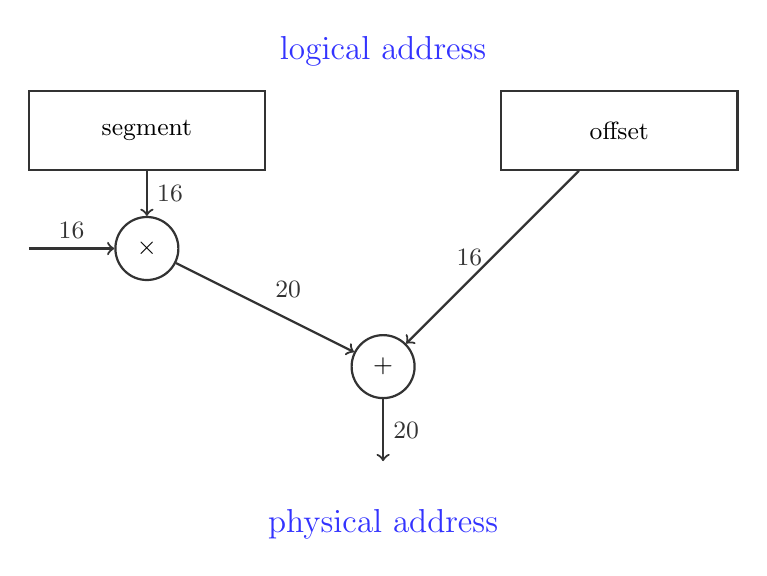
\begin{tikzpicture}[
    font=\small,
    box/.style={draw=black!80, thick, rectangle, minimum width=3cm, minimum height=1cm},
    circ/.style={draw=black!80, thick, circle, minimum size=8mm},
    arrow/.style={->, thick, black!80}
]

% Titles
\node[font=\large, blue!80] at (0,4) {logical address};

% Boxes
\node[box] (segment) at (-3,3) {segment};
\node[box] (offset)  at ( 3,3) {offset};

% Operators
\node[circ] (mul) at (-3,1.5) {$\times$};
\node[circ] (add) at ( 0,0) {$+$};

% Physical address
\node[font=\large, blue!80] at (0,-2) {physical address};

% Arrows
\draw[arrow] (segment) -- node[right] {16} (mul);
\draw[arrow] (mul) -- node[above right] {20} (add);
\draw[arrow] (offset) -- node[left] {16} (add);
\draw[arrow] (add) -- node[right] {20} (0,-1.2);

% Extra input to multiplier (shift left by 4)
\draw[arrow] (-4.5,1.5) -- node[above] {16} (mul);

\end{tikzpicture}
	\end{center}
Now if we take a look at the protected mode (80286), now we have a sort of multiprogramming.


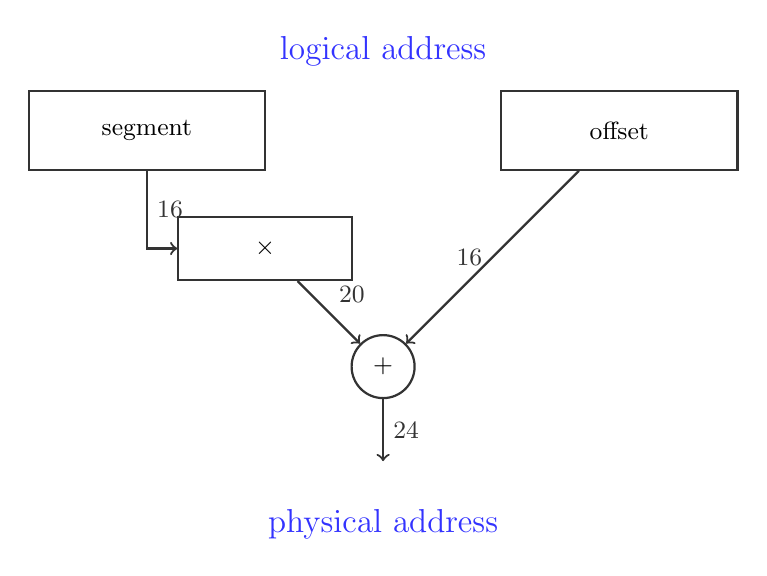
\begin{tikzpicture}[
    font=\small,
    box/.style={draw=black!80, thick, rectangle, minimum width=3cm, minimum height=1cm},
    opbox/.style={draw=black!80, thick, rectangle, minimum width=2.2cm, minimum height=0.8cm},
    circ/.style={draw=black!80, thick, circle, minimum size=8mm},
    arrow/.style={->, thick, black!80}
]

% Title
\node[font=\large, blue!80] at (0,4) {logical address};

% Boxes
\node[box] (segment) at (-3,3) {segment};
\node[box] (offset)  at ( 3,3) {offset};

% Operators
\node[opbox] (mul) at (-1.5,1.5) {$\times$};
\node[circ]  (add) at ( 0,0) {$+$};

% Physical address
\node[font=\large, blue!80] at (0,-2) {physical address};

% Arrows
\draw[arrow] (segment) -- node[right] {16} (-3, 1.5) -- (mul);
\draw[arrow] (mul) -- node[above right] {20} (add);
\draw[arrow] (offset) -- node[left] {16} (add);
\draw[arrow] (add) -- node[right] {24} (0,-1.2);


\end{tikzpicture}

Now if we go even later in the protected mode (80386, 80486, Plentium). we need now to have a bit of multiprogramming right?
\begin{center}
    \includegraphics[scale=0.25]{screenshots/2025-12-16_5.png}
\end{center}




\end{parag}

\begin{parag}{Operand Types}
    \begin{itemize}
		\item \important{Not} a load/store architecture
    \end{itemize}
	\begin{center}
	\begin{tabular}{|c|c|}
		Source 1 = Destination & Source 2 \\
		\hline
		Register & Register \\
		\hline
		Register & Immediate \\
		\hline
		Register & Memory \\
		\hline
		Memory & Register \\
		\hline
		Memory & Immediate \\
		\hline
	    
	\end{tabular}
	\end{center}
	Immediate values can be on 8, 16, or 32 bits.
	
    
\end{parag}

\begin{parag}{Addressing Mode I}
   \begin{itemize}
	   \item \important{Absolute}
	   \item \important{Register indirect} \textrightarrow $\left[\text{reg}\right]$
		   \begin{itemize}
			   \item 16-bit registers : \texttt{BX}, \texttt{SI}, \texttt{DI} 
			   \item 32-bit registers: \texttt{EAX}, \texttt{ECX}, \texttt{EDX}, \texttt{EBX}, \texttt{ESI}, \texttt{EDI}
		   \end{itemize}
	   \item \important{Displacement} \textrightarrow [reg + displacement]
		   \begin{itemize}
			   \item 16-bit registers: \texttt{BP}, \texttt{BX}, \texttt{SI}, \texttt{DI}
			   \item 32-bit registers: \texttt{EAX}, \texttt{ECX}, \texttt{EDX}, \texttt{EBX}, \texttt{ESI}, \texttt{EDI}
			   \item Displacement on 8, 16, or 32 bits
		   \end{itemize}
	   \item \important{Indexed} \textrightarrow [bas reg + reg]
		   \begin{itemize}
			   \item 16-bit registers: \texttt{BX} + \texttt{SI}, \texttt{BX} + \texttt{DI}, \texttt{BP} + \texttt{SI}, \texttt{BP} + \texttt{DI}
		   \end{itemize}
   \end{itemize}
    
\end{parag}


\begin{parag}{Addressing Mode II}
    \begin{itemize}
		\item \important{Indexed with displacement} \textrightarrow [base + reg + reg + displacement]
			\begin{itemize}
				\item Same registers as in mode indexed
			\end{itemize}
		\item \important{Scaled indexed} \textrightarrow $\left[\text{base reg + }2^{\text{scale}}x \; \text{reg}\right]$
			\begin{itemize}
				\item Only in 32 bit mode
				\item Scale is 0, 2, or 3
				\item Index register can be any of the basic registers (except ESP)
				\item Base register can be any of the basic registers
			\end{itemize}
		\item \important{Scaled indexed with displacement} \textrightarrow 
			\begin{align*} 
			\left[\text{base reg } + 2^{\text{scale}}x \text{ reg } + \text{displacement}\right]
			\end{align*}
    \end{itemize}
\end{parag}

\begin{parag}{Address Segment (Legacy)}
	For every indirect addressing (e.g., [reg]) the appropriate segment would be needed to complete the address\\
	Default:
	\begin{itemize}
		\item Regerences to instructions (\texttt{IP}) use \texttt{CS} (code segment register)
		\item References to stack (\texttt{BP} or \texttt{SP}) use \texttt{SS} (stack segement register)
		\item All other references use \texttt{DS} (data segement register)
	\end{itemize}
	A \important{one-byte instruction prefix} can modify the default
\end{parag}
\begin{parag}{A Growing ISA}
	\begin{itemize}
		\item \important{80386} (1985): 32-bit registers, flat memory model, paging, and virtual memory
		\item  \important{80486} (1989): x87 floating-point coprocessor instructions integrated
		\item  \important{MMX} (1997): SIMD instructions for multimedia (8-bit, 16-bit, 32-bit integer)
		\item  \important{SSE} (1999): 128-bit SIMD for floating-point, integer, and memory operations
		\item  \important{SSE2} (2001): Double-precision floating-point and integer operations
		\item  \important{SSE3/SSSE3} (2004-2006): Minor enhancements (e.g., horizontal add/subtract)
		\item  \important{SSE4} (2007-2008): Adds text processing (SSE4.2) and improved vector processing
		\item  \important{AVX} (2011): 256-bit SIMD, non-destructive 3-operand form, VEX prefix
		\item  \important{AVX2} (2013): Adds integer operations, gathers, and FMA (Fused Multiply-Add)
		\item  \important{AVX-512} (2016): 512-bit SIMD, mask registers, expanded precision operations
		\item  \important{x86-64} (2003, \important{AMD}): 64-bit, more registers (R8–R15), RIP-relative addressing
	\end{itemize}
    
\end{parag}



\begin{parag}{Number of x86 instructions over time}
	\begin{center}
	\includegraphics[scale=0.25]{screenshots/2025-12-16_6.png}
	\end{center}
\end{parag}
\begin{parag}{Instruction Examples}
\end{parag}
\begin{tabular}{>{\ttfamily}l p{10cm}}
\hline
\textbf{Instruction} & \textbf{Description} \\
\hline
JE addr & if equal(CC) then IP $\leftarrow$ addr (IP-128 $\le$ addr < IP+128) \\
JMP addr & IP $\leftarrow$ addr \\
CALL addr,seg & SP $\leftarrow$ SP-2; Mem[SS:SP] $\leftarrow$ IP+5 \\
 & SP $\leftarrow$ SP-2; Mem[SS:SP] $\leftarrow$ CS \\
 & IP $\leftarrow$ addr; CS $\leftarrow$ seg \\
MOVW BX,[DI+45] & BX $\leftarrow$ Mem[DS:DI+45] \\
PUSH SI & SP $\leftarrow$ SP-2; Mem[SS:SP] $\leftarrow$ SI \\
POP DI & DI $\leftarrow$ Mem[SS:SP]; SP $\leftarrow$ SP+2 \\
ADD AX,#6765 & AX $\leftarrow$ AX + 6765 \\
TEST DX,#42 & set CC flags with (DX and 42) \\
MOVSB & Mem[ES:DI] $\leftarrow$ Mem[DS:SI]; DI $\leftarrow$ DI+1; SI $\leftarrow$ SI+1 \\
\hline
\end{tabular}
\begin{parag}{Instruction Encoding}
    As we have seen before, instruction doesn't have a fixed size, so how do we encode?
	\begin{itemize}
		\item One instruction coded on 1 to 17 bytes
		\item Several types of modifiers/predixes
		\item Two combinations of constants of variable length 
			\begin{itemize}
				\item Immediate and Displacement
				\item 8, 16, and 32-bit
			\end{itemize}
		\item Opcode "lost" and only moderately orthogonal
	\end{itemize}
	\begin{center}
		\includegraphics[scale=0.2]{screenshots/2026-02-07.png}
	\end{center}	
	For instance here are some instructions and their encodings:
	\begin{center}
	\includegraphics[scale=0.25]{screenshots/2026-02-07_1.png}
	\end{center}
\end{parag}
\begin{parag}{Improved Encoding and Generality}
    Here if we take the legacy \texttt{MUL} instruction encoded as \texttt{0xF7 E3}  (16 bits)
	\begin{lstlisting}
MOV RAX, 5  ; Load first operand into RAX (implicit source)
MOV RBX, 10  ; Load second operand into RBX
MUL RBX ; Multiply RAX * RBX  -> result in RDX:RAX
	\end{lstlisting}
	As we can see there is a lot of implicit information for each instruction:
	\begin{itemize}
		\item The multiplier is \important{implicit} (it's always in the \texttt{RAX} register)
		\item Multiplicand is \important{explicit} 
		\item The result is stored in two register: \texttt{RAX} gets the lower bits, \texttt{RDX} gets the higher bits
	\end{itemize}
	Now if we take the modern \texttt{MULX} instruction, it is encoded as \texttt{0xF2 0F 38 F6} (32 bits)
	\begin{lstlisting}
MOV RAX, 5  ; Load first operand into RAX (explicitly  RAX, required)
MOV RBX, 10  ; Load second operand into RBX
MUL RDX, RCX, RBX ; Multiply RBX * RAX -> RCX = low, RDX = high
	\end{lstlisting}
	Now the result has to be specified.
\end{parag}
\begin{parag}{1995:PentiumPro (P6) A Superscalar x86 CISC?}
	How to adapt the superscalar ideas to fit such an irregular architecture?
	\begin{itemize}
		\item The complexity of decoding is huge
		\item Parallel decoding of instructions is tough due to an encoding strongly variable in length 
		\item Instructions mix memory operations with computations
		\item Too few registers
	\end{itemize}
\end{parag}
\begin{parag}{PentiumPro Microarchitecture: Out-of-order CISC Execution}
	So how do we do it? We split our architecture in two parts: the decoder which translate from CISC instruction to RISC. then we issue all the 'risc' instruction to our classic RISC processor:

\end{parag}
	\begin{center}
	\includegraphics[scale=0.3]{screenshots/2026-02-07_2.png}
	\end{center}
	\begin{parag}{PentiumPro In-Order Section}
	    \begin{itemize}
			\item Converts every x86 instruction into one or more internal RISC-like 118-bit instructions (micro-operations or uops); on average 1 instruction = 1.5-2 uops
			\item Three decoders and a sequencer work in parallel to perform the conversion
				\begin{itemize}
					\item Two highest priority simple decoders intercept register-register operations (1 instr. \textrightarrow 1 uop)
					\item A low priority general decoder handles all other basic operations (1 instr. \textrightarrow 1 uop)
					\item A low priority general decoder handles all other basic operations (1 instr. \textrightarrow 4 uops)
					\item A sequencer is used by the general decoder for very complex operations (1 instr \textrightarrow several groups of 4 uops)
				\end{itemize}
			\item Reorder Buffer (ROB) implements renaming and commits uops in program order to the Real Register File (RRF)
	    \end{itemize}
	    
	\end{parag}
	\begin{parag}{PentiumPro Out-of-order Section}
	Superscalar is very similar to the general model studied in previous lessons:
	\begin{itemize}
		\item Up to 20 uops wait in the Reservation Stations until the operands are all available
		\item A maximum of 5 uops can be issued per cycle: a generic calculation (int or FP), a simple integer (no shift, mul nor div), a load, a store address, and a store data
		\item A Memory Reorder Buffer (MOB) reorders memory accesses and waits for D-cache availability
	\end{itemize}
	
	\end{parag}
	
	\begin{framedremark}
	For the rest of the lecture there is a lot of examples so I will show some of them but not all
	\end{framedremark}

	\begin{parag}{Pentium 4: Processors for the Multi-GHz Era}
 Intel had introduced IA-64 (Itanium) for high-performance computing, however the Pentium line continued evolving to achieve very high clock frequencies. The Pentium 4 was designed with several features to reach multi-GHz operation:

\begin{itemize}
    \item \important{Deep pipeline:} The Pentium 4 extended the pipeline to \important{20 stages} (compared to 10 in Pentium III) to allow shorter clock cycles and higher frequencies. Each stage performs simpler operations, reducing the critical path delay.
    \item \important{Wire delays handled explicitly:} Dedicated pipeline stages were introduced to manage wire propagation delays, which become significant at multi-GHz frequencies.
    \item \important{Trace caches:} Stores approximately 12,000 decoded micro-operations (uops) to avoid repeatedly decoding x86 instructions in the main loop, effectively acting as an L0 cache for uops.
    \item \important{Out-of-order execution:} Up to 126 uops can be in-flight simultaneously, allowing the processor to schedule independent instructions efficiently.
    \item \important{Data speculation:} The processor may execute loads before stores speculatively. If a true dependence exists, the load is squashed and replayed.
    \item \important{ALU throughput:} Simple arithmetic and logic operations can be executed in half a clock cycle. This allows two dependent instructions to be scheduled in the same cycle, improving overall throughput.
\end{itemize}

\end{parag}

\begin{parag}{Simultaneous Multi-Threading: Xeon Pipeline}
	\begin{center}
	\includegraphics[scale=0.3]{screenshots/2026-02-07_3.png}
	\end{center}
    
\end{parag}


	





\subsection{Conclusions}
\begin{itemize}
	\item x86 is the oldest important ISA around
	\item It is not absolutely fixed but a family of constantly evolving ISAs with many new addons (MMX, SSE, AVX, CMOV, etc.)
	\item Intel has managed to continue pushing the performance by adapting to its CISC nature the techniques developed to speed-up newer RISC processors
\begin{itemize}
	\item Similar work has been done by some competitors—notably by AMD with Athlon, for a few months the fastest x86 processor on the market
\end{itemize}
	\item  It has been given for agonizing many times over, it is still well alive and kicking!...
\end{itemize}

